\section{D. 소가 길을 건너간 이유 2020}

\begin{frame} % No title at first slide
    \sectiontitle{D}{소가 길을 건너간 이유 2020}
    \sectionmeta{
        \texttt{dynamic\_programming}\\
        출제진 의도 -- \textbf{\color{acplatinum}Medium}
    }
    \begin{itemize}
        \item 제출 270번, 정답 30팀 (정답률 11.11\%)
        \item 처음 푼 팀: \textbf{Let Us Win UCPC 2020} (윤교준, 김세빈, 이민제), 27분
        \item 출제자: \texttt{functionx}
    \end{itemize}
\end{frame}

\begin{frame}{\textbf{D}. 소가 길을 건너간 이유 2020}
    \begin{center}
        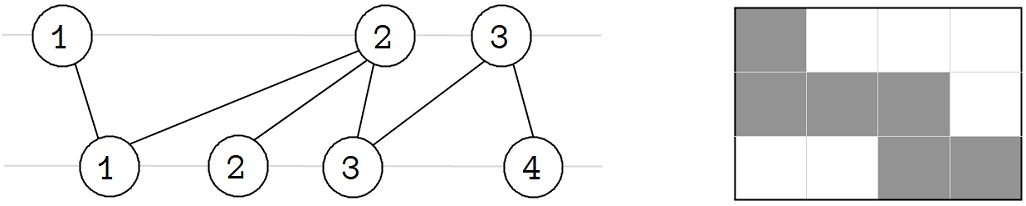
\includegraphics[width=0.8\linewidth]{../images/cow-fly/D-1.png}
    \end{center}
    \begin{itemize}
        \item $N \times M$ 격자를 그려봅시다.
        \item 위쪽 $i$번째 헛간과 아래쪽 $j$번째 헛간을 연결하는 항로가 있다면 격자의 $i$행 $j$열을 칠해줍시다.
        \item 놀랍게도 1행 1열에서 $N$행 $M$열까지 가는 최단경로 형태가 됩니다.
    \end{itemize}
\end{frame}

\begin{frame}{\textbf{D}. 소가 길을 건너간 이유 2020}
    \begin{center}
        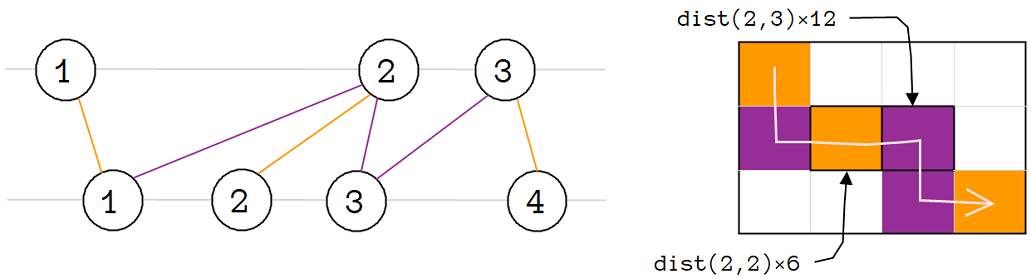
\includegraphics[width=0.8\linewidth]{../images/cow-fly/D-2.png}
    \end{center}
    \begin{itemize}
        \item 역발상을 해보자면, 최단거리의 합은 각 항로에 대하여 (항로의 힘) × (항로를 지나는 경로의 수)의 합입니다.
        \item (항로를 지나는 경로의 수)는 $N+M-1$ 또는 $(i+j-1)(N+M-i-j+1)$입니다.
        \item 격자에서 보면 직진할 때는 $N+M-1$, 꺾을 때는 $(i+j-1)(N+M-i-j+1)$입니다.
    \end{itemize}
\end{frame}

\begin{frame}{\textbf{D}. 소가 길을 건너간 이유 2020}
    DP 정의를 이렇게 합니다.
    \begin{itemize}
        \item $DP[i][j][dir]$ : 격자의 $i$행 $j$열 까지 간 다음 dir(오른쪽/아래쪽) 방향으로 나갈 때 최소비용
        \item $i$행 $j$열을 지난 이후의 상황은 무시합니다.
    \end{itemize}
    \vspace{0.2in}
    $(i,j)$ 직전에 어디를 지났는지 생각해보면 점화식을 세울 수 있습니다.
\end{frame}